\documentclass{../../../oss-apphys}
%\usepackage{bm}
%\usepackage{wrapfig}

\begin{document}
\genheader

\gentitle{1}{WORK AND ENERGY}

\genmultidirections

\gengravity

\raggedcolumns
\begin{multicols}{2}

  \begin{enumerate}[leftmargin=18pt]

  \item A \SI{1}{\kilo\gram} ball is thrown vertically downward from a
    $50$-meter-high tower with an initial speed of \SI{4}{\metre\per\second}.
    Just before striking the ground, the speed of the ball is
    \SI{20}{\metre\per\second}. The energy lost to air friction is most nearly
    \begin{enumerate}[nosep,label=(\Alph*)]
      \item\SI{101}{\joule}
      \item\SI{210}{\joule}
      \item\SI{308}{\joule}
      \item\SI{406}{\joule}
      \item\SI{508}{\joule}
    \end{enumerate}
  \end{enumerate}

  
  \textbf{Questions \ref{q:pq1}--\ref{q:pq2}}. A \SI{2}{\kilo\gram} projectile
  is launched with a speed of \SI{20}{\metre\per\second} from horizontal ground
  at an angle of \ang{37} to the horizontal as shown. Point $P$ is at the top
  of the path, and point $Q$ is at the end of the path, just before the
  projectile again reaches the ground.
  \begin{center}
    \pic{.35}{symprojectile.png}
  \end{center}
  \begin{enumerate}[leftmargin=18pt,resume]
  \item The kinetic energy of the projectile at point $P$ is
    \label{q:pq1}
    \begin{enumerate}[nosep,label=(\Alph*)]
    \item\SI{108}{\joule}
    \item\SI{225}{\joule}
    \item\SI{256}{\joule}
    \item\SI{400}{\joule}
    \item\SI{525}{\joule}
    \end{enumerate}
    
  \item The kinetic energy of the projectile at point $Q$ is
    \label{q:pq2}
    \begin{enumerate}[nosep,label=(\Alph*)]
    \item\SI{108}{\joule}
    \item\SI{225}{\joule}
    \item\SI{256}{\joule}
    \item\SI{400}{\joule}
    \item\SI{525}{\joule}
    \end{enumerate}
    \columnbreak
    
%A toy train car of mass 3.0 kg rolls to the left at 2 m/s and collides with
%a 4.0 kg train car rolling to the right at 1 m/s. The two cars stick
%together. The velocity of the cars after the collision is
%(A) 2/7 m/s to the left
%(B) 2/7 m/s to the right
%(C) 4/7 m/s to the left
%(D) 4/7 m/s to the right
%(E) 9/7 m/s to the right

    %MAY BE THIS ONE
%  \item Two steel balls, one of mass m and the other of mass 2m, collide and
%    rebound in a perfectly elastic collision. Which of the following is
%    conserved in this elastic collision?
%(A) velocity only
%(B) momentum only
%(C) momentum and kinetic energy only
%(D) momentum, velocity, and kinetic energy(E) kinetic energy only
%Questions 153–154. A force acts on a 2.0 kg mass during a time interval as
%shown in the graph.
%153. The impulse given to the mass from t = 0 to t = 6 s is
%(A) 4 N s
%(B) 8 N s
%(C) 12 N s
%(D) 16 N s
%(E) 24 N s
%154. If the initial speed of the mass is 2 m/s at t = 0, what is its speed at the
%end of 6 s?
%(A) 4 m/s
%(B) 6 m/s
%(C) 8 m/s
%(D) 10 m/s
%    %(E) 16 m/s
%  \item A rubber ball of mass $m$ strikes a wall with a speed $v$ at an angle
%    $\theta$ below the normal line and rebounds from the wall at the same speed
%    and angle above the normal line as shown. The change in momentum
%    of the ball is
%    \begin{center}
%      \pic{.25}{graphics/ball-bounce-wall.png}
%    \end{center}
%    \begin{enumerate}[nosep,label=(\Alph*)]
%    \item $mv$
%    \item $2mv$
%    \item $mv\cos\theta$
%    \item $2mv\cos\theta$
%    \item  zero
%    \end{enumerate}
%    
%156. Two blocks are connected by a compressed spring and rest on a
%frictionless surface. The blocks are released from rest and pushed apart
%by the compressed spring. If one mass is twice the mass of the other,
%which of the following is the same for both blocks?
%(A) magnitude of momentum
%(B) acceleration
%(C) speed
%(D) kinetic energy
%(E) potential energy
%  \item A \SI{1000}{\kilo\gram} railroad car is rolling without friction on a
%    horizontal track at a speed of \SI{3.}{\metre\per\second}. Sand is poured
%    into the open top of the car for a time of \SI{5.}{\second}. The speed of
%    the car after \SI{5.}{\second} is \SI{1.}{\metre\per\second}. The mass of
%    the sand added to the car at the end of \SI{5.}{\second} is
%    \begin{center}
%      \pic{.25}{graphics/railroad-car-sand.png}
%    \end{center}
%    \begin{enumerate}[nosep,label=(\Alph*)]
%    \item\SI{500 }{\kilo\gram}
%    \item\SI{1000}{\kilo\gram}
%    \item\SI{2000}{\kilo\gram}
%    \item\SI{3000}{\kilo\gram}
%    \item\SI{3500}{\kilo\gram}
%    \end{enumerate}
%    \columnbreak
%    
%  \item Two billiard balls are rolling to the right on a table as shown. The
%    \SI{.4}{\kilo\gram} ball is moving faster than the \SI{.2}{\kilo\gram}
%    ball, so it catches up and strikes it from behind at a slight angle.
%    Immediately after the collision, the $y$-component of the
%    \SI{.4}{\kilo\gram} ball is \SI{2}{\metre\per\second} downward.
%    The $y$-component of the velocity of the \SI{.2}{\kilo\gram} ball must be
%    \begin{center}
%      \pic{.25}{graphics/big-small-billiard-balls.png}
%    \end{center}
%    \begin{enumerate}[nosep,label=(\Alph*)]
%    \item \SI{1}{\metre\per\second} upward
%    \item \SI{2}{\metre\per\second} upward
%    \item \SI{1}{\metre\per\second} downward
%    \item \SI{2}{\metre\per\second} downward
%    \item \SI{4}{\metre\per\second} upward
%    \end{enumerate}
%    
%Questions 159–160. Two balls are on a horizontal billiard table. A 1.0 kg
%billiard ball moves downward along the y-axis with a speed of 16 m/s toward
%a 2.0 kg ball that is at rest. The balls collide at an angle, and move along the
%lines shown. After the collision, the 1.0 kg ball moves at 9 m/s along the +x-
%axis. The table below shows the x and y components of the momentum in kg
%m/s of the two balls before and after the collision.
%159. Which of the following statements is true?
%(A) Momentum is conserved only in the x-direction in this collision.
%(B) Momentum is conserved only in the y-direction in this collision.
%(C) Momentum is conserved in both the x- and y-directions in this
%collision
%(D) The momentum of the 1.0 kg ball increases after the collision.
%(E) The momentum of the 2.0 kg ball decreases after the collision.160. What is the speed of the 2.0 kg ball after the collision?
%(A) 16.0 m/s
%(B) 9.2 m/s
%(C) 7.5 m/s
%(D) 6.0 m/s
%(E) 5.0 m/s
%161. A 0.3 kg baseball at rest on a tee is struck by a bat. The ball leaves the
%bat with a speed of 20 m/s at an angle of 45° above the horizontal. The
%magnitude of the impulse imparted to the baseball by the bat is most
%nearly
%(A) 2 N s
%(B) 6 N s
%(C) 12 N s
%(D) 16 N s
%(E) 20 N s
%162. Two ice skaters, a large man and a small woman, are initially at rest
%and holding each other’s hands. They push away horizontally.
%Afterward, which of the following statements is true?
%(A) They have equal and opposite kinetic energies.
%(B) The have equal and opposite momenta.
%(C) The large man applies a greater force to the small woman.
%(D) The small woman applies a greater force to the large man.
    %(E) They recoil with equal and opposite velocities.
%
%  \end{enumerate}
%  \columnbreak
%  
%  \textbf{Questions 4-5}
%
%  An object has a mass $4m$. The object explodes into three pieces of mass
%  $m$, $m$, and $2m$. The two pieces of mass m move off at right
%  angles to each other with the same momentum $mv$, as shown.
%  \begin{center}
%    \pic{.25}{graphics/3-piece-bomb.png}
%  \end{center}
%  \begin{enumerate}[leftmargin=18pt,resume]
%  \item The speed of mass 2m after the explosion is
%    \begin{enumerate}[nosep,label=(\Alph*)]
%    \item $2v$
%    \item $\sqrt{2}v$
%    \item $\frac{\sqrt{2}}{2}v$
%    \item $\frac{\sqrt{2}}{3}v$
%    \item $\frac{\sqrt{3}}{2}v$
%    \end{enumerate}
%    
%  \item  The direction of velocity of mass $2m$ is
%    \begin{enumerate}[nosep,label=(\Alph*)]
%    \item $\rightarrow$
%    \item $\swarrow$
%    \item $\downarrow$
%    \item $\nearrow$
%    \item $\uparrow$
%    \end{enumerate}
%  \end{enumerate}
%165. A system consists of two blocks having masses of 2 kg and 1 kg. Theblocks are connected by a string of negligible mass and hung over a
%light pulley, and then released from rest. When the speed of each block
%is v, the momentum of the center of mass of the system is
%(A) (2 kg + 1 kg)v
%(B) (2 kg - 1 kg)v
%(C) 1/3 (2 kg + 1 kg)v
%(D) 1⁄2 (2 kg - 1 kg)v
%(E) (2 kg)v
%
%  \columnbreak
%  \textbf{Questions 6-7}
%
%  A projectile is launched at an angle to the level ground as shown. At the top
%  of the trajectory at point $P$, the projectile explodes into two pieces of
%  mass $2m$ and $m$.
%  \begin{center}
%    \pic{.25}{graphics/exploding-projectile.png}
%  \end{center}
%
%  \begin{enumerate}[leftmargin=18pt,resume]
%  \item Which of the following arrows best represents the direction of the
%    velocity of the center of mass of the projectile at point $P$ after the
%    explosion?
%    \begin{enumerate}[nosep,label=(\Alph*)]
%    \item $\leftarrow$
%    \item $\swarrow$
%    \item $\searrow$
%    \item $\rightarrow$
%    \item $\nearrow$
%    \end{enumerate}
%
%  \item Which of the following statements is true of the center of mass of the
%    projectile after the explosion?
%    \begin{enumerate}[nosep,label=(\Alph*)]
%    \item The center of mass will continue on a parabolic path and land on
%      the ground at the place where it would have landed had it not exploded.
%    \item The center of mass will alter its parabolic path and land on the
%      ground farther from where it would have landed had it not exploded.
%    \item The center of mass will alter its parabolic path and land on the
%      ground at a shorter distance than it would have landed had it not
%      exploded.
%    \item The center of mass will fall straight downward from the point of
%      explosion.
%    \item The center of mass will travel straight upward from the point of
%      explosion.
%    \end{enumerate}
%    
%Questions 168–169. Two pieces of clay of equal mass m moving with equal
%speeds v o each traveling at an angle of 30° collide and stick together at the
%origin O as shown.
%168. Which of the following arrows represents the direction of the velocity
%of the combined mass after the collision?
%(A)
%(B)
%(C)
%(D)
%(E)
%169. The speed of the combined mass after the collision is
%(A) v o
%(B) 1⁄2 v o
%(C) 1⁄4 v o(D)
%(E)
%    \columnbreak
%    
%  \item A small mass $m$ is moving with a speed $v$ toward a stationary mass
%    $2m$. The speed of the center of mass of the system is
%    \begin{enumerate}[nosep,label=(\Alph*)]
%    \item $\displaystyle\left(\frac{m}{m+2m}\right)v$
%    \item $\displaystyle\left(\frac{m+2m}{m}\right)v$
%    \item $\displaystyle\left(\frac{m}{2m}\right)v$
%    \item $\displaystyle\left(1+\frac{m}{2m}\right)v$
%    \item $\displaystyle\left(1+\frac{32m}{m}\right)v$
%    \end{enumerate}
%  \end{enumerate}
%  
%  \textbf{Questions 9-10}
%
%  Three identical masses can slide freely on a horizontal surface as shown.
%  The first mass moves with a speed of 3.0 m/s toward the second and third
%  masses, which are initially at rest. The first and second mass collide
%  elastically, and then the second and third masses collide inelastically.
%  \begin{center}
%    \pic{.4}{graphics/3-masses.png}
%  \end{center}
%
%  \begin{enumerate}[leftmargin=18pt,resume]
%  \item The speed of the second mass after the collision is
%    \begin{enumerate}[nosep,label=(\Alph*)]
%    \item zero
%    \item\SI{1.5}{\metre\per\second}
%    \item\SI{3.}{\metre\per\second}
%    \item\SI{6.}{\metre\per\second}
%    \item\SI{9.}{\metre\per\second}
%    \end{enumerate}
%
%  \item The speed of the second and third masses after they collide
%    inelastically is
%    \begin{enumerate}[nosep,label=(\Alph*)]
%    \item zero
%    \item\SI{1.5}{\metre\per\second}
%    \item\SI{3.0}{\metre\per\second}
%    \item\SI{6.0}{\metre\per\second}
%    \item\SI{9.0}{\metre\per\second}
%    \end{enumerate}
%    
%173. The diagram in the figure shows the top view of two identical steel
%balls on a horizontal table of negligible friction. The first ball moves
%with a speed of 12 m/s and the second ball is initially at rest. After the
%collision, the first ball moves with a speed of 8 m/s at an angle of 37°
%to the vertical. Which of the following diagrams best represents the
%approximate speed and direction of the second ball after the collision?
%(A)(B)
%(C)
%(D)
%(E)
%174. A known force F acts on an unknown mass for a known time Δt. From
%this information, you could determine the
%(A) change in kinetic energy of the object
%(B) change in velocity of the object
%(C) acceleration of the object
%(D) mass of the object
%(E) change in momentum of the object175. A block of mass m is moving to the right with a speed v o on a
%horizontal surface of negligible friction when it explodes. The
%explosion causes the block to break into two pieces, each of which
%moves in the horizontal direction. One piece of mass m/4 moves to the
%left with a speed of 2v o . What is the velocity of the other piece?
%(A)
%(B)
%(C)
%(D)
%(E)
%2v o to the right
%v o to the right
%3⁄4 v o to the right
%1⁄2 v o to the right
%1⁄4 v o to the left
%Questions 176–177. The graph shown indicates the force acting on a mass of
%2 kg as a function of time.
%176. For the time interval from t = 0 to t = 6 s, the change in momentum of
%the 2 kg mass is
%(A) 48 kg m/s
%(B) 24 kg m/s
%(C) 12 kg m/s
%(D) -12 kg m/s
%(E) zero
%177. If the object starts from rest, the speed at the end of the time interval
%from t = 0 to t = 3 s is
%(A) zero(B)
%(C)
%(D)
%(E)
%12 m/s
%18 m/s
%24 m/s
%36 m/s
%    \columnbreak
%    
%  \item A \SI{100}{\kilo\gram} cannon sits at rest with a \SI{1}{\kilo\gram}
%    cannonball in the barrel. The cannonball is fired with a speed of
%    \SI{50}{\metre\per\second} to the right, causing the cannon to recoil with
%    a speed of \SI{.5}{\metre\per\second} to the left. The velocity of the
%    center of mass of the cannon-cannonball system is
%    \begin{enumerate}[nosep,label=(\Alph*)]
%    \item zero
%    \item\SI{5}{\metre\per\second} to the right
%    \item\SI{5}{\metre\per\second} to the left
%    \item\SI{50}{\metre\per\second} to the right
%    \item\SI{50}{\metre\per\second} to the left
%    \end{enumerate}
%    
%179. The vector shown represents the initial momentum of a moving object.
%The object collides with another object that is initially at rest. Which of
%the diagrams below could represent the momenta of the colliding
%objects after the collision?
%(A)
%(B)
%(C)
%(D)
%(E)
%Questions 180–181. A 20 kg boy runs at a speed of 3.0 m/s and jumps onto a
%40 kg sled on frictionless ice that is initially at rest. The boy and the sled then
%move together for a short time.
%180. The speed of the boy and sled after he jumps on it is
%(A) 0.5 m/s(B)
%(C)
%(D)
%(E)
%0.8 m/s
%1.0 m/s
%1.5 m/s
%2.0 m/s
%181. While the boy and sled are moving, he jumps off the back of the sled in
%such a way the boy is at rest, and the sled continues to move forward.
%The speed of the sled after the boy jumps off is
%(A) 1.5 m/s
%(B) 2.0 m/s
%(C) 3.0 m/s
%(D) 4.5 m/s
%(E) 6.0 m/s
%Questions 182–183
%A cart of mass m 1 is initially moving with a speed of 4.0 m/s on a track
%toward a stationary cart of mass m 2 = 2 kg. After the collision, mass m 1
%moves with a velocity of 1.5 m/s. The force vs. time graph is shown for the
%time during the collision, with the collision beginning at t = 0.
%182. The impulse each cart applies to the other is most nearly
%(A) 40 N s
%(B) 20 N s
%(C) 10 N s
%(D) 5 N s(E) 2 N s
%183. The unknown mass m 1 is equal to
%(A)
%(B)
%(C)
%(D)
%(E)
%0.5 kg
%1.5 kg
%2.5 kg
%4.0 kg
%5.0 kg
%184. A 1.0 kg block is released from rest from a height h at the top of a
%fixed curved ramp of negligible friction. The block slides down the
%ramp and collides with another block of mass 1.5 kg at rest at the
%bottom of the ramp. The two blocks stick together and move with a
%speed of 5 m/s. The height h from which the 1.0 kg block began is
%(A) 0.8 m
%(B) 1.2 m
%(C) 1.8 m
%(D) 2.8 m
%(E) 7.8 m
%185. A dart of mass m is fired into a wooden block of mass 4m that hangs
%from a string. The dart and block then rise to a maximum height h. An
%expression for the initial speed v o of the dart before striking the block is
%(A)
%(B)
%(C)
%(D)
%(E)Questions 186–187. A small block of mass m slides on a horizontal
%frictionless surface toward a ramp of mass 3m which is also free to move on
%the surface. The small block slides up to a height h on the ramp with no
%friction (Figure I), then they move together (Figure II), and the small block
%slides back down the ramp to the horizontal surface (Figure III). Both the
%block and the ramp continue to slide on the horizontal surface after they
%separate.
%186. Which of the following is true regarding the conservation laws
%throughout this process?
%(A) Kinetic energy is conserved from Figure I to Figure II.
%(B) Momentum is conserved from Figure I to Figure III.
%(C) Kinetic energy is conserved from Figure II to Figure III.
%(D) Potential energy is conserved from Figure I to Figure II.
%(E) Potential energy is conserved from Figure II to Figure III.
%187. Which of the following is a true statement regarding Figure III?
%(A) The small block is moving to the left and the ramp is moving to
%the right.
%(B) The small block is moving to the right and the ramp is moving to
%the left.
%(C) The small block is moving to the right and the ramp is moving tothe right.
%(D) The small block is moving to the left and the ramp is moving to
%the left.
%(E) The small block and the large block are moving with the same
%velocity.
%Questions 188–189. A rubber ball of mass m is released from rest from a
%height h onto a fixed inclined plane angled at 45° to the horizontal. The ball
%collides with the surface elastically.
%188. Which of the following diagrams best indicates the direction of the
%impulse vector J as it strikes the plane and the velocity vector v just
%after it strikes the plane?
%(A)
%(B)
%(C)
%(D)
%(E)
%189. The speed of the ball just after striking the surface is(A)
%(B)
%(C)
%(D)
%(E)
%
%  \item A \SI{1000}{\kilo\gram} (empty mass) railroad car is rolling without
%    friction on a horizontal track at a speed of \SI{2.}{\metre\per\second}.
%    Sand is poured into the open top of the car for the time interval from
%    $t=0$ to $t=\SI{4.}{\second}$. The mass of the sand poured into the car as
%    a function of time is $m(t)=60t^2$. The velocity of the car at a time of
%    \SI{4.}{\second} is most nearly
%    \begin{center}
%      \pic{.25}{graphics/railroad-car-sand.png}
%    \end{center}
%    \begin{enumerate}[nosep,label=(\Alph*)]
%    \item\SI{1}{\metre\per\second}
%    \item\SI{2}{\metre\per\second}
%    \item\SI{3}{\metre\per\second}
%    \item\SI{4}{\metre\per\second}
%    \item\SI{5}{\metre\per\second}
%    \end{enumerate}
%  \end{enumerate}
%  \columnbreak
%  
%  \textbf{Questions 13-14}
%
%  A remote controlled stunt car of mass \SI{800}{\kilo\gram} initially moving at
%  \SI{10}{\metre\per\second} is crashed into a rail car of mass $m$ that is
%  initially at rest. The cars stick together, and the speed $v$ of both cars
%  after the collision is given by $\displaystyle v=\frac{6}{t+1}$.
%  \begin{enumerate}[resume,leftmargin=18pt]
%  \item By considering the fact that the crash occurs at time $t=0$, determine
%    the mass $m$ of the rail car.
%    \begin{enumerate}[nosep,label=(\Alph*)]
%    \item\SI{288}{\kilo\gram}
%    \item\SI{445}{\kilo\gram}
%    \item\SI{533}{\kilo\gram}
%    \item\SI{698}{\kilo\gram}
%    \item\SI{800}{\kilo\gram}
%    \end{enumerate}
%    
%  \item The magnitude of the resisting force acting on the cars as a function of
%    time after the collision is
%    \begin{enumerate}[nosep,label=(\Alph*)]
%    \item $\displaystyle \frac{6m}{t+1}$
%    \item $6m(t+1)$
%    \item $6m(t+1)^2$
%    \item $\displaystyle\frac{6m}{(t+1)^2}$
%    \item $\displaystyle\frac{m(t+1)^2}{6}$
%    \end{enumerate}
%    
%193. A force acts on a mass m according to the equation F = 12t 3 . If the
%object starts from rest, the velocity of the object as a function of time is
%(A) 36mt 3
%(B)
%(C)
%(D)
%(E)
%194. A dart in a long blow gun starts from rest and gains a momentum
%according to the equation p = 3t 3 + 2t while moving through the barrel
%of the gun. The net force acting on the dart after 0.2 s is
%(A) 1.2 N
%(B) 2.4 N
%(C) 6.0 N(D) 12.2 N
%(E) 16.1 N
%195. A variable force acts on a mass causing it to accelerate. If a graph of
%this force vs. time is plotted, the change in momentum of the mass can
%be determined by finding the
%(A) slope of the graph
%(B) area under the graph
%(C) y-intercept of the graph
%(D) x-intercept of the graph
%(E) change in slope of the graph
%196. A moving object is changing its momentum during a time interval. If a
%graph of momentum vs. time is plotted, the net force acting on the mass
%at any time can be determined by finding the
%(A) slope of line tangent to the graph at that time
%(B) area under the graph
%(C) y-intercept of the graph
%(D) x-intercept of the graph
%(E) change in slope of the graph from beginning to end
%
%
%  \item Two masses moving along the coordinates axes as shown collide at the
%    origin and stick to each other. What is the angle $\theta$ that the final
%    velocity that makes with the $x$-axis?
%    \begin{center}
%      \pic{.28}{collision1.png}
%    \end{center}
%
%    \begin{enumerate}[nosep,label=(\Alph*)]
%    \item $\tan^{-1}(v_2/v_1)$
%    \item $\tan^{-1}[m_1v_1/(m_1+m_2)]$
%    \item $\tan^{-1}(m_1v_2/m_2v_1)$
%    \item $\tan^{-1}(m_2v_2^2/m_1v_1^1)$
%    \item $\tan^{-1}(m_2v_2/m_1v_1)$
%    \end{enumerate}
%    \columnbreak
    
  \item If a projectile thrown directly upward reaches a maximum height $h$ and
    spends a total time in the air of $T$, the average power of the
    gravitational force during the trajectory is
    \begin{enumerate}[nosep,label=(\Alph*)]
    \item $P=2mgh/T$
    \item $P=-2mgh/T$
    \item 0
    \item $P=mgh/T$
    \item $P=-mgh/T$
    \end{enumerate}

  \item Given that the constant net force on an object and the object's 
    displacement, which of the following quantities can be calculated?
    \begin{enumerate}[nosep,label=(\Alph*)]
    \item the net change in the object's velocity
    \item the net change in the object's mechanical energy
    \item the average acceleration
    \item the net change in the object's kinetic energy
    \item the net change in the object's potential energy
    \end{enumerate}
    \vspace{.8in}
    
  \item An electron travels in a circle around a hydrogen nucleus at a very high
    speed. The work done by the electrostatic force acting on the electron
    after one complete revolution is
    \begin{enumerate}[nosep,label=(\Alph*)]
    \item zero
    \item positive
    \item negative
    \item equal to the kinetic energy of the electron
    \item equal to the potential energy of the electron
    \end{enumerate}
    \columnbreak
    
  \item An object is moved from rest at point $P$ to rest at point $Q$ in a
    gravitational field. The net work against the gravitational field depends
    on the
    \begin{enumerate}[nosep,label=(\Alph*)]
    \item mass of the object and the positions of $P$ and $Q$
    \item mass of the object only
    \item positions of $P$ and $Q$ only
    \item length moved between points $P$ and $Q$
    \item coefficient of friction
    \end{enumerate}
    \vspace{.8in}
%  \end{enumerate}
%  
%  \textbf{Questions \ref{q:well1}--\ref{q:well2}}. Consider the potential energy
%  function shown below.
%  \begin{center}
%    \pic{.28}{potential-well.png}
%  \end{center}
%  \begin{enumerate}[resume,leftmargin=18pt]
%  \item Assuming that no non-conservative forces are present, if a particle of
%    mass $m$ is released from position $x_0$, what is the maximum speed it will
%    achieve?
%    \label{q:well1}
%    \begin{enumerate}[nosep,label=(\Alph*)]
%    \item $\sqrt{4U_0/m}$
%    \item $\sqrt{2U_0/m}$
%    \item $\sqrt{U_0/m}$
%    \item $\sqrt{U_0/2m}$
%    \item The particle will achieve no maximum speed but instead will continue
%      to accelerate indefinitely.
%    \end{enumerate}
%
%  \item Which of the following is the most accurate description of the system
%    introduced in the previous question?
%    \label{q:well2}
%    \begin{enumerate}[nosep,label=(\Alph*)]
%    \item stable equilibrium
%    \item unstable equilibrium
%    \item neutral equilibrium
%    \item a bound system
%    \item There is a linear restoring force
%    \end{enumerate}
  
%  \item A mass $m_1$ initially moving at speed $v_0$ collides with and sticks
%    to a spring attached to a second, initially stationary mass $m_2$. The two
%    masses continue to move to the right on a frictionless surface as the
%    length of the spring oscillates. At the instant that the spring is
%    maximally extended, the velocity of the first mass is
%    \begin{center}
%      \pic{.35}{mass-spring-1.png}
%    \end{center}
%    \begin{enumerate}[nosep,label=(\Alph*)]
%    \item $v_0$
%    \item $m_1^2v_0/(m_1+m_2)^2$
%    \item $m_2v_0/m_1$
%    \item $m_1v_0/m_2$
%    \item $m_1v_0/(m_1+m_2)$
%    \end{enumerate}
%    \columnbreak
    
  \item A pendulum bob of mass $m$ is released from rest as shown in the figure
    below. What is the tension in the string as the pendulum swings through the
    lowest point of its motion?
    \begin{center}
      \begin{tikzpicture}[scale=.95]
        \draw[dashed](0,0)--(0,-3.5);
        \begin{scope}[rotate=60]
          \draw(0,0)--(0,-4);
          \fill[black](0,-4) circle(.13) node[right]{\tiny $m$};
          \draw[<->](.5,0)--(.5,-4) node[midway,above right]{\tiny $l$};
        \end{scope}
        \draw[<->](0,-1)arc(270:330:1) node[pos=.6,below]{\tiny\ang{60}};
      \end{tikzpicture}
    \end{center}
    \begin{enumerate}[nosep,label=(\Alph*)]
    \item $\displaystyle T=\frac{1}{2}mg$
    \item $T=mg$
    \item $\displaystyle T=\frac{3}{2}mg$
    \item $T=2mg$
    \item None of the above
    \end{enumerate}
    \columnbreak
    
  \item Two blocks of mass $m_A$ and $m_B$ are connected by a string that
    passes over a light pulley. The mass of $A$ is larger than the mass of $B$.
    The speed of mass $A$ just before reaching the floor is:
    \begin{center}
      \pic{.18}{pulley-a-b.png}
    \end{center}
    \begin{enumerate}[nosep,label=(\Alph*)]
    \item $\displaystyle\sqrt{\frac{m_A-m_B}{m_A+m_B}gD}$
    \item $\displaystyle\sqrt{\frac{m_A+m_B}{m_A-m_B}gD}$
    \item $\displaystyle\sqrt{\frac{m_A}{m_A+m_B}gD}$
    \item $\displaystyle\sqrt{\frac{m_B}{m_A+m_B}gD}$
    \item $\displaystyle\sqrt{\frac{m_A}{m_B}gD}$
    \end{enumerate}
  \end{enumerate}
  \columnbreak
  
  \textbf{Questions \ref{q:down1}--\ref{q:down2}}. A force is applied to a block
  of mass $m$ at a downward angle of $\theta$ to the vertical as shown. The
  block moves with a constant speed across a rough floor for a distance $x$.
  \begin{center}
    \pic{.3}{downward-angle.png}
  \end{center}
  \begin{enumerate}[resume,leftmargin=18pt]
  \item The work done by the applied force on the block is
    \label{q:down1}
    \begin{enumerate}[nosep,label=(\Alph*)]
    \item $Fx\sin\theta$
    \item $Fx\cos\theta$
    \item $Fmx\sin\theta$
    \item $Fmx\cos\theta$
    \item zero
    \end{enumerate}
    
  \item The coefficient of friction between the block and the floor is
    \label{q:down2}
    \begin{enumerate}[nosep,label=(\Alph*)]
    \item $\displaystyle\frac{F}{mg}$
    \item $\displaystyle\frac{F\cos\theta}{mg}$
    \item $\displaystyle\frac{F\cos\theta}{F\sin\theta+mg}$
    \item $\displaystyle\frac{F\sin\theta}{F\cos\theta+mg}$
    \item $\displaystyle\frac{F\cos\theta}{F\sin\theta}$
    \end{enumerate}
  \end{enumerate}
  \columnbreak
  
  \textbf{Questions \ref{sphere1}--\ref{sphere2}}. A small block rests on the
  top of a smooth sphere of radius $R$ when it is given a light tap so that it
  just begins sliding on the sphere. When the block reaches the angle $\theta$,
  it loses contact with the surface of the sphere.
  \begin{center}
    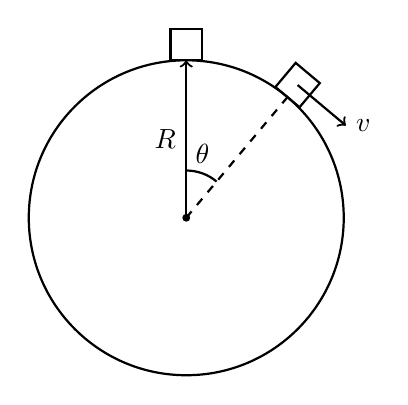
\begin{tikzpicture}
      \draw[thick](0,0) circle(2);
      \fill(0,0) circle(.05);
      \draw[thick,->](0,0)--(0,2) node[midway,left]{$R$};
      \draw[thick](-.2,2) rectangle(.2,2.4);
      \begin{scope}[rotate around={-40:(0,0)}]
        \draw[thick,dashed](0,0)--(0,2);
        \draw[thick](-.2,2) rectangle(.2,2.4);
        \draw[->,thick](0,2.2)--(.8,2.2) node[pos=1,right]{$\mb{v}$};
      \end{scope}
      \draw[thick](0,.6) arc(90:50:.6) node[midway,above]{$\theta$};
    \end{tikzpicture}
  \end{center}  
  \begin{enumerate}[resume,leftmargin=18pt]
  \item The kinetic energy of the block as it leaves the surface of the sphere
    is
    \label{sphere1}
    \begin{enumerate}[nosep,label=(\Alph*)]
    \item $mgR$
    \item $mgR\cos\theta$
    \item $mgR\sin\theta$
    \item $mg(R-R\cos\theta)$
    \item $mg(R-R\sin\theta)$
    \end{enumerate}

  \item The speed of the block as it leaves the surface of the sphere is
    \label{sphere2}
    \begin{enumerate}[nosep,label=(\Alph*)]
    \item $\displaystyle\sqrt{2g}{m}$
    \item $\displaystyle\sqrt{2gR}{m}$
    \item $\displaystyle 2gR\cos\theta$
    \item $\displaystyle 2g(R-R\cos\theta)$
    \item $\displaystyle 2g(R-R\sin\theta)$
    \end{enumerate}
    
  \item A small ball starts from rest and rolls down a quarter-circle ramp of
    radius $R$. The speed of the ball at the point halfway down the ramp is
    most nearly
    \begin{center}
      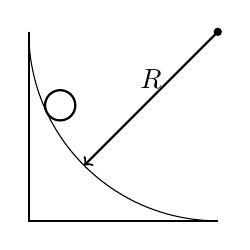
\begin{tikzpicture}[scale=2.4]
        \draw[thick](-1,0)--(-1,-1)--(0,-1);
        \draw(-1,0) arc(180:270:1);
        \draw[thick,->,rotate=45](0,0)--(-1,0) node[midway,above,sloped]{$R$};
        \draw[thick,rotate=25](-.92,0) circle(.08);
        \fill (0,0) circle(.022);
      \end{tikzpicture}
    \end{center}
    \begin{enumerate}[nosep,label=(\Alph*)]
    \item $gR$
    \item $2gR$
    \item $\displaystyle\sqrt{gR\sin\ang{45}}$
    \item $\displaystyle\sqrt{2gR\sin\ang{45}}$
    \item The speed cannot be determined without knowing the mass of the ball.
    \end{enumerate}
  \end{enumerate}
\end{multicols}
\newpage

\genfreetitle{1}{WORK AND ENERGY}{5}

\genfreedirections

% TAKEN FROM 2005 AP PHYSICS B EXAM, FREE-RESPONSE QUESTION #2
\begin{center}
  \pic{.45}{pendulum.png}
\end{center}

\begin{enumerate}[leftmargin=15pt]
\item A simple pendulum consists of a bob of mass 1.8 kg attached to a string
  of length 2.3 m. The pendulum is held at an angle of \ang{30} from the
  vertical by a light horizontal string attached to a wall, as shown above.
  \begin{enumerate}[leftmargin=18pt,resume]
  \item On the figure below, draw a free-body diagram showing and labeling the
    forces on the bob in the position shown above.
    \begin{center}
      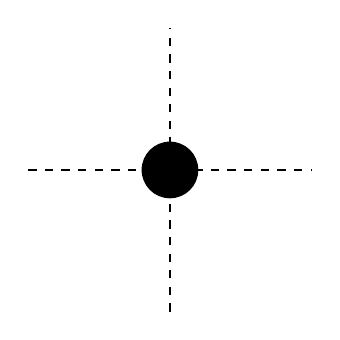
\begin{tikzpicture}[scale=.9]
        \draw[dashed](-2,0)--(2,0);
        \draw[dashed](0,-2)--(0,2);
        \fill(0,0) circle(.4);
      \end{tikzpicture}
    \end{center}
  \item Calculate the tension in the horizontal string.
  \item The horizontal string is now cut close to the bob, and the pendulum
    swings down. Calculate the speed of the bob at its lowest position.
  \end{enumerate}
  \newpage
  
  \begin{center}
    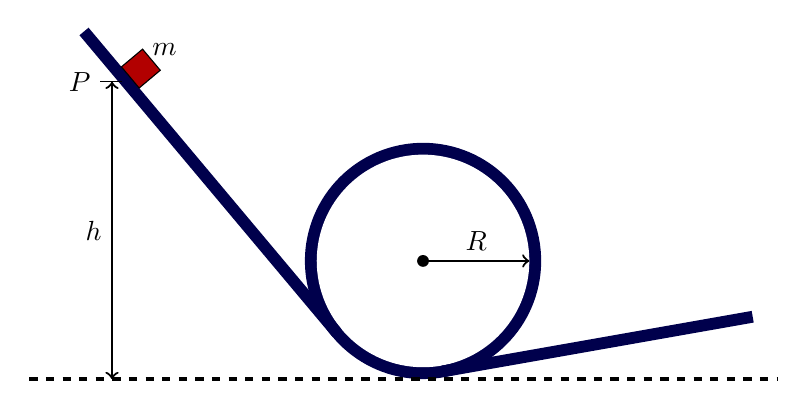
\begin{tikzpicture}[scale=.5]
      \fill[blue!30!black](0,0) circle(3);
      \fill[white](0,0) circle(2.7);
      \fill[black](0,0) circle(.15);
      \draw[thick,->](0,0)--(2.7,0) node[midway,above]{$R$};
      \begin{scope}[rotate=10]
        \fill[blue!30!black](0,-2.7) rectangle(8,-3);
      \end{scope}
      \begin{scope}[rotate=-50]
        \fill[blue!30!black](0,-2.7) rectangle(-10,-3);
        \fill[red!70!black,draw=black](-8,-2.7) rectangle(-8.7,-2)
        node[right,black]{$m$};
      \end{scope}
      \draw[dashed,very thick](-10,-3)--(9,-3);
      \draw[thick,<->](-7.9,-3)--(-7.9,4.55) node[midway,left]{$h$};
      \draw(-7.65,4.55)--(-8.2,4.55) node[pos=1,left]{$P$};    
    \end{tikzpicture}
  \end{center}
\item A small block of mass $m$ slides without friction along the loop-the-loop
  track shown in the figure above. The block starts from point $P$ a distance
  $h$ above the bottom of the loop.
  \begin{enumerate}[noitemsep]
  \item What is the kinetic energy of the block when it reaches the top of
    the loop?
  \item What is the acceleration at the top of the loop, assuming that it
    stays on the track?
  \item What is the least value of $h$ for which the block will reach the top
    of the loop without leaving the track?
  \end{enumerate}
  \newpage
  
\item A $2.0$-\si{\kilo\gram} block is released \SI{4.}{\metre} from a massless
  spring with a spring constant of \SI{100}{\newton\per\metre} that is fixed
  along a frictionless plane inclined at \ang{30}, as shown in the figure below.
  Plese give answer to $3$ significant figures.
  \begin{center}
    \begin{tikzpicture}[scale=.7]
      \begin{scope}[rotate=-30]
        \fill(0,0) rectangle(-.1,1);
        \draw[thick,
          decoration={aspect=.4,segment length=1.5mm, amplitude=2mm,coil},
          decorate] (-.1,.5)--(-1.5,.5)
        node[midway,above right]{$k=\SI{100}{\newton\per\metre}$};
        \fill(-1.5,0) rectangle(-1.6,1);
        \draw[<->,thick](-1.6,1.5)--(-5.6,1.5)
        node[midway,above right,sloped]{\SI{4.}{\metre}};
        \draw[thick](-1.6,1.05)--(-1.6,2);
        \draw[thick](-5.6,1.05)--(-5.6,2);
        \draw[fill=yellow!50](-5.6,0) rectangle(-6.3,.7)
        node[black,above left]{$m=\SI{2.}{\kilo\gram}$};
      \end{scope}
      \draw[fill=pink!50](0,0)--(-6.06,0)--(-6.06,3.5)--cycle;
      \draw[<->,thick](-2,0) arc(180:150:2) node[midway,left]{\ang{30}};
    \end{tikzpicture}
  \end{center}
  \begin{enumerate}[noitemsep,leftmargin=20pt]
  \item Find the maximum compression of the spring.
  \item If the plane is not frictionless, and the coefficient of kinetic
    friction between it and the block is $0.20$, find the maximum compression.
  \item For the rough incline ($\mu=0.20$), how far up the incline will the
    block travel after leaving the spring?
  \end{enumerate}
  \newpage

  \begin{center}
    \pic{.8}{table}
  \end{center}
\item A physics class is asked to design a low-friction slide that will launch
  a block horizontally from the top of a lab table. Teams 1 and 2 assemble the
  slides shown above and use identical blocks 1 and 2, respectively. Both
  slides start at the same height d above the tabletop. However, team 2's table
  is lower than team 1's table. To compensate for the lower table, team 2
  constructs the right end of the slide to rise above the tabletop so that the
  block leaves the slide horizontally at the same height h above the floor as
  does team 1's block (see figure above).
  \begin{enumerate}[noitemsep,leftmargin=20pt]
  \item Both blocks are released from rest at the top of their respective
    slides. Do block 1 and block 2 land the same distance from their respective
    tables?

    \vspace{.1in}
    \underline{\hspace{.3in}} Yes\hspace{.2in}
    \underline{\hspace{.3in}} No

    \vspace{.1in}Justify your answer.\vspace{.4in}
  \end{enumerate}
  \newpage
  
  In another experiment, teams 1 and 2 use tables and low-friction slides with
  the same height. However, the two slides have different shapes, as shown
  below.
  \begin{center}
    \pic{.8}{table2}
  \end{center}
  \begin{enumerate}[noitemsep,leftmargin=20pt,resume]
  \item Both blocks are released from rest at the top of their respective
    slides at the same time.
    \begin{enumerate}[noitemsep,leftmargin=18pt]
    \item Which block, if either, lands farther from its respective table?

      \vspace{.1in}
      \underline{\hspace{.3in}} Block 1
      \underline{\hspace{.3in}} Block 2
      \underline{\hspace{.3in}} The two blocks land the same distance from
      their respective tables.

      \vspace{.1in}Briefly explain your reasoning without manipulating
      equations.\vspace{\stretch{1}}
    \item Which block, if either, hits the floor first?

      \vspace{.1in}
      \underline{\hspace{.3in}} Block 1
      \underline{\hspace{.3in}} Block 2
      \underline{\hspace{.3in}} The two blocks hit the floor at the same time.

      \vspace{.1in}Briefly explain your reasoning without manipulating
      equations.\vspace{\stretch{1}}
    \end{enumerate}
  \end{enumerate}
  \newpage
  
\item A pendulum of length $L$ has a bob of mass $m$. It is released from some
  angle $\theta_1$. The string hits a peg at a distance $x$ directly below the
  pivot, as shown in the figure below, effectively shortening the length of the
  pendulum. Find the maximum angle $\theta_2$ between the string and the
  vertical when the bob is to the right of the peg.
  \begin{center}
    \pic{.4}{pendulum-peg}
  \end{center}
  

\end{enumerate}
\end{document}
